\section{Crowding distance. NSGA-II.}
Crowding distance для двумерного случая:\\
$\frac{dx}{DX} + \frac{dy}{DY}$
\begin{figure}[!ht]
$x$ - текущее решение
$y$ - доминирующее множество 

Подсчёт расстояния происходит следующим образом: идёт сортировка по первхой координате и смотрим на 2-ух соседей, затем смотрим на размах фронта по этой координате ($x$), нормируем его ($DX$) прибавляем, и так же итеративно по всем координатам.

Чем больше расстояние - тем больше расстояние до соседей, тем меньше хочется удалять точку (решение). Если решение попало на край фронта, тогда его ценность - бесконечна
\begin{center}
    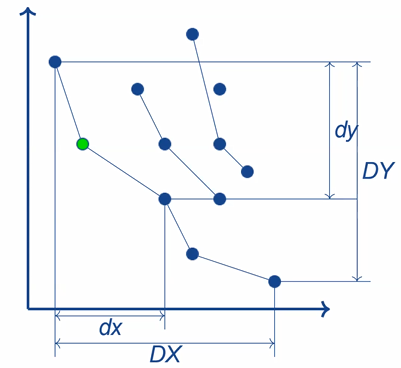
\includegraphics[width=0.8\linewidth]{images/Crowding_distance.PNG}
    \caption{Crowding distance для двумерного случая}
    \label{fig:mpr}
    
\end{center}
\end{figure}

Схема алгоритма NSGA-II\\

Параметры:\\
- Размер популяции N, число критериев K, собственно критерии\\
- Операторы скрещивания и мутации\\

Схема\\
Начало: Порождаем N случайных решений, вычисляем приспособленность,
определяем ранги и crowding distance внутри каждого ранга\\
На каждой итерации:\\
1) Порождаем N/2 пар решений, каждое решение выбираем турнирным отбором\\
- Турнир: сначала сравниваем по рангу, потом по crowding distance. Чем меньше ранг - тем лучше, при одинаковых рангах чем больше crowding distance - тем лучше\\
- Хитрая группировка решений: каждое участвует ровно в двух турнирах. Если решения будут участвовать более чем в 2 турнирах, тогда решения каждый раз будут переопределяться, что помешает ранжированию собоственно по crowding distance на предыдущем этапе. Поэтому на предыдущем рисунке crowding distance зелёной точки только для 2-ух!! соседних точек\\
2) Проводим скрещивание и мутацию, вычисляем приспособленность\\
3) Сваливаем старых и новых особей в кучу, выбираем N лучших. Сравнение не проводится по функции приспособленности, т.к. этим действием мы сократим разнообразие в турнирном отборе\\
- Сначала сравниваем решения по рангу, потом по crowding distance\\

 В целом значимость NSGA-II можно объяснить так: у нас есть модель для ГА, которая сходится в глобальном оптимуме. Эта модель модифицируется с помощью NSGA-II, где происходит ранжирование для отбора оптимальных, т.е. задача оптимизации для решения задачи оптимизации)).
